\documentclass{beamer}
\usepackage[utf8]{inputenc}
\usepackage{subfiles}
\usepackage{lipsum}
\usepackage{float}
\usepackage{listings}
\usepackage{color}
\usepackage{tikz}
\usepackage{lmodern}
\usepackage{algorithmic}

\definecolor{darkblue}{rgb}{0.086,0.145,0.357}
\definecolor{darkpurple}{rgb}{0.3098,0 , 0.3098}
\definecolor{skinorange}{rgb}{0.957,0.639 , 0.365}


\usetikzlibrary{arrows.meta,arrows}
\usetikzlibrary{positioning}

\usetheme{Madrid}
\usecolortheme{beaver}

\title[Priority Queue]{Priority Queue}
\subtitle{A brief Overview}
\author[Awsaf, Fuad] % (optional, for multiple authors)
{Md Awsaf Alam\inst{1} \and \\Ahmed Nafis Fuad\inst{1}}
\institute[BUET] % (optional)
{
  \inst{1}%
  Department of Computer Science and Engineering\\
  BUET
}
\date{\today}


\AtBeginSection[]{
\begin{frame}
    \tableofcontents[currentsection]
\end{frame}
}

\begin{document}
\titlepage

\begin{frame}{Table of Contents}
\tableofcontents

\end{frame}

\section{What is a Priority Queue?}
\subfile{sec/definition.tex}


\section{Example of Priority Queue}
\subfile{sec/application.tex}

\section{Applications of Priority Queue}
\begin{frame}{Applications}
\begin{itemize}
  \item  Dijkstra’s Shortest Path Algorithm using priority queue: When the graph is stored in the form of adjacency list or matrix, priority queue can be used to extract minimum efficiently when implementing Dijkstra’s algorithm. \pause
  \item  Prim’s algorithm: It is used to implement Prim’s Algorithm to store keys of nodes and extract minimum key node at every step. \pause
  \item  Data compression : It is used in Huffman codes which is used to compresses data. \pause
  \item  CPU scheduling : Each queue may have its own scheduling algorithm, implemented using priority queue.
\end{itemize}

\end{frame}


\section{Implementations of Priority Queue}
\begin{frame}{Implementations of Priority Queue}
\setbeamercovered{dynamic}
\centering
Priority Queues can be implemented using : \pause
\begin{itemize}
  \item Fibonacci Heap \pause
  \item Binary Heap \pause
\end{itemize}

\end{frame}

\section{Binary Max Heap}
\begin{frame}{Definition}
  A Binary (Max) Heap is a complete binary tree that maintains the Max Heap property.
  Binary Heap is one possible data structure to model an efficient Priority Queue. \pause
  \begin{itemize}
    \item The largest element in a max-heap is stored at the root
    \item Each node of the tree corresponds to an element of the array that
stores the value in the node. \pause
    \item The tree is completely filled on all levels except possibly the
lowest, where it is filled from the left up to a point.
  \end{itemize}
\end{frame}
\begin{frame}{Representing Binary Heap as an array}
  \begin{columns}
    \column{0.45\textwidth}
    \begin{enumerate}
      \item The root node is A[1] \onslide<1->
      \item Node i is A[i] \onslide<2->
      \item The parent of node i is A[i/2] \onslide<3->
      \item The left child of node i is A[2i] \onslide<4->
      \item The right child of node i is A[2i + 1] \onslide<5->
    \end{enumerate}
    \column{0.5\textwidth}
      \begin{center} \onslide<1->
        \tikzset{every picture/.style={line width=0.75pt}} %set default line width to 0.75pt

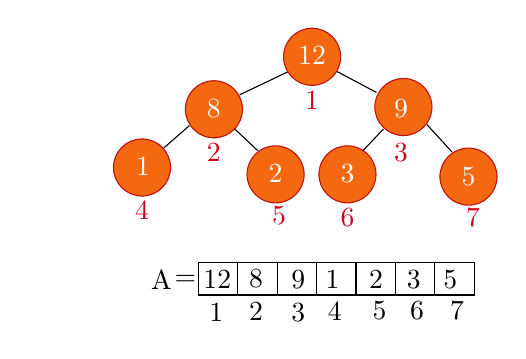
\begin{tikzpicture}[x=0.75pt,y=0.75pt,yscale=-0.55,xscale=0.55]
%uncomment if require: \path (0,300); %set diagram left start at 0, and has height of 300

\draw  [color={rgb, 255:red, 189; green, 19; blue, 19 }  ,draw opacity=1 ][fill={rgb, 255:red, 244; green, 105; blue, 16 }  ,fill opacity=1 ]  (321, 32) circle [x radius= 25, y radius= 25]  ;
\draw  [color={rgb, 255:red, 189; green, 19; blue, 19 }  ,draw opacity=1 ][fill={rgb, 255:red, 244; green, 105; blue, 16 }  ,fill opacity=1 ]  (235, 78) circle [x radius= 25, y radius= 25]  ;
\draw    (257.5,65.33) -- (299.5,45.33) ;


\draw  [color={rgb, 255:red, 189; green, 19; blue, 19 }  ,draw opacity=1 ][fill={rgb, 255:red, 244; green, 105; blue, 16 }  ,fill opacity=1 ]  (401, 76) circle [x radius= 25, y radius= 25]  ;
\draw    (343,45) -- (377.5,63.33) ;


\draw  [color={rgb, 255:red, 189; green, 19; blue, 19 }  ,draw opacity=1 ][fill={rgb, 255:red, 244; green, 105; blue, 16 }  ,fill opacity=1 ]  (172, 129) circle [x radius= 25, y radius= 25]  ;
\draw    (191,112) -- (213.5,92.33) ;


\draw  [color={rgb, 255:red, 189; green, 19; blue, 19 }  ,draw opacity=1 ][fill={rgb, 255:red, 244; green, 105; blue, 16 }  ,fill opacity=1 ]  (289, 135) circle [x radius= 25, y radius= 25]  ;
\draw    (253,95) -- (273.5,114.33) ;


\draw  [color={rgb, 255:red, 189; green, 19; blue, 19 }  ,draw opacity=1 ][fill={rgb, 255:red, 244; green, 105; blue, 16 }  ,fill opacity=1 ]  (352, 135) circle [x radius= 25, y radius= 25]  ;
\draw    (365.5,114.33) -- (383.5,95.33) ;


\draw  [color={rgb, 255:red, 189; green, 19; blue, 19 }  ,draw opacity=1 ][fill={rgb, 255:red, 244; green, 105; blue, 16 }  ,fill opacity=1 ]  (458, 137) circle [x radius= 25, y radius= 25]  ;
\draw    (421.5,91.33) -- (443.5,115.33) ;


\draw    (290.5, 212) rectangle (325, 240.67)   ;
\draw    (394, 212) rectangle (428.5, 240.67)   ;
\draw    (359.5, 212) rectangle (394, 240.67)   ;
\draw    (221.5, 212) rectangle (256, 240.67)   ;
\draw    (256, 212) rectangle (290.5, 240.67)   ;
\draw    (428.5, 212) rectangle (463, 240.67)   ;
\draw    (325, 212) rectangle (359.5, 240.67)   ;

\draw (321,31) node [color={rgb, 255:red, 255; green, 255; blue, 255 }  ,opacity=1 ] [align=left] {12};
\draw (321,70) node [color={rgb, 255:red, 208; green, 2; blue, 27 }  ,opacity=1 ] [align=left] {1};
\draw (235,77) node [color={rgb, 255:red, 255; green, 255; blue, 255 }  ,opacity=1 ] [align=left] {8};
\draw (235,116) node [color={rgb, 255:red, 208; green, 2; blue, 27 }  ,opacity=1 ] [align=left] {2};
\draw (399,77) node [color={rgb, 255:red, 255; green, 255; blue, 255 }  ,opacity=1 ] [align=left] {9};
\draw (399,116) node [color={rgb, 255:red, 208; green, 2; blue, 27 }  ,opacity=1 ] [align=left] {3};
\draw (173,128) node [color={rgb, 255:red, 255; green, 255; blue, 255 }  ,opacity=1 ] [align=left] {1};
\draw (172,167) node [color={rgb, 255:red, 208; green, 2; blue, 27 }  ,opacity=1 ] [align=left] {4};
\draw (86,174) node [color={rgb, 255:red, 255; green, 255; blue, 255 }  ,opacity=1 ] [align=left] {1};
\draw (250,174) node [color={rgb, 255:red, 255; green, 255; blue, 255 }  ,opacity=1 ] [align=left] {5};
\draw (289,134) node [color={rgb, 255:red, 255; green, 255; blue, 255 }  ,opacity=1 ] [align=left] {2};
\draw (292,171) node [color={rgb, 255:red, 208; green, 2; blue, 27 }  ,opacity=1 ] [align=left] {5};
\draw (352,134) node [color={rgb, 255:red, 255; green, 255; blue, 255 }  ,opacity=1 ] [align=left] {3};
\draw (352,173) node [color={rgb, 255:red, 208; green, 2; blue, 27 }  ,opacity=1 ] [align=left] {6};
\draw (290,185) node [color={rgb, 255:red, 255; green, 255; blue, 255 }  ,opacity=1 ] [align=left] {1};
\draw (367,231) node [color={rgb, 255:red, 255; green, 255; blue, 255 }  ,opacity=1 ] [align=left] {5};
\draw (458,137) node [color={rgb, 255:red, 255; green, 255; blue, 255 }  ,opacity=1 ] [align=left] {5};
\draw (462,173) node [color={rgb, 255:red, 208; green, 2; blue, 27 }  ,opacity=1 ] [align=left] {7};
\draw (189,228) node  [align=left] {A};
\draw (210,228) node  [align=left] {=};
\draw (238,227) node  [align=left] {12};
\draw (272,226) node  [align=left] {8};
\draw (309,227) node  [align=left] {9};
\draw (339,227) node  [align=left] {1};
\draw (377,227) node  [align=left] {2};
\draw (410,227) node  [align=left] {3};
\draw (442,227) node  [align=left] {5};
\draw (237,256) node  [align=left] {1};
\draw (272,255) node  [align=left] {2};
\draw (309,256) node  [align=left] {3};
\draw (448,254) node  [align=left] {7};
\draw (413,254) node  [align=left] {6};
\draw (380,254) node  [align=left] {5};
\draw (341,255) node  [align=left] {4};


\end{tikzpicture}
      \end{center}
  \end{columns}

\end{frame}

\subfile{sec/tree_animation.tex}

\section{Algorithm}
\subfile{sec/algorithm.tex}

\begin{frame}
  \frametitle{Analysing Running Time}
  Extract Max : $O(1)$ \newline
  Heapify:
  $T(n) \leq T(2n/3) \plus O(1)$ \newline
  Solving the recurrence, we have
  $T(n) = O(lg n)$ \newline
  Thus, Heapify() takes $O(h)$ time for a node at height h.
\end{frame}

\section{Conclusion}
\begin{frame}{The End}
  \begin{center}
    Any Questions?
  \end{center}
\end{frame}
\end{document}
